% C.23 菱形，对角线 6, 8
\documentclass[tikz,border=4pt]{standalone}
\usepackage{ctex}
\usepackage{amsmath}
\usetikzlibrary{calc, arrows.meta,decorations.markings}
\begin{document}
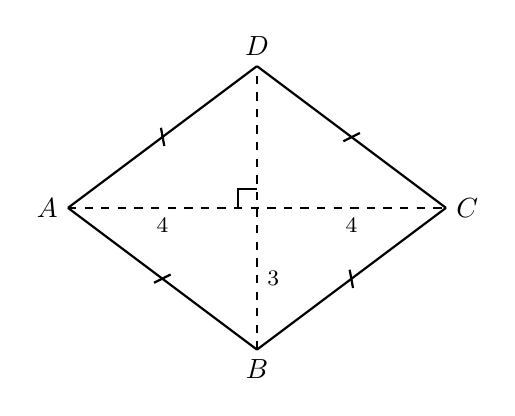
\begin{tikzpicture}[scale=0.6, thick,
  tickone/.style={postaction={decorate, decoration={markings,
    mark=at position 0.5 with {\draw (-1.5pt,-3pt) -- (1.5pt,3pt);}}}}]
  \coordinate (A) at (-4,0);
  \coordinate (C) at (4,0);
  \coordinate (B) at (0,-3);
  \coordinate (D) at (0,3);
  \draw[tickone] (A) -- (B);
  \draw[tickone] (B) -- (C);
  \draw[tickone] (C) -- (D);
  \draw[tickone] (D) -- (A);
  \draw[dashed] (A) -- (C);
  \draw[dashed] (B) -- (D);
  \draw (-0.4,0) -- (-0.4,0.4) -- (0,0.4);
  \node[left] at (A) {$A$};
  \node[right] at (C) {$C$};
  \node[below] at (B) {$B$};
  \node[above] at (D) {$D$};
  \node[font=\footnotesize, below] at (-2,0) {$4$};
  \node[font=\footnotesize, below] at (2,0) {$4$};
  \node[font=\footnotesize, right] at (0,-1.5) {$3$};
\end{tikzpicture}
\end{document}
